\documentclass[12pt,twoside]{article}
\usepackage{amsmath, amssymb}
\usepackage{amsmath}
\usepackage[active]{srcltx}
\usepackage{amssymb}
\usepackage{amscd}
\usepackage{makeidx}
\usepackage{amsthm}
\usepackage{algpseudocode}
\usepackage{algorithm}
\usepackage{graphicx}
\renewcommand{\baselinestretch}{1}
\setcounter{page}{1}
\setlength{\textheight}{21.6cm}
\setlength{\textwidth}{14cm}
\setlength{\oddsidemargin}{1cm}
\setlength{\evensidemargin}{1cm}
\pagestyle{myheadings}
\thispagestyle{empty}
\markboth{\small{Josu\'e David Hern\'andez Ram\'irez}}{\small{.}}
\date{}
\begin{document}
\centerline{\bf Ingeniería de Software, Sem: 2021-1, 3CV3, Tarea 1, 07/11/2020}
\centerline{}
\centerline{}
\begin{center}
\Large{\textsc{Tarea 2: Administración de proyectos}}
\end{center}
\centerline{}
\centerline{\bf {Josu\'e David Hern\'andez Ram\'irez.}}
\centerline{}
\centerline{Escuela Superior de C\'omputo}
\centerline{Instituto Polit\'ecnico Nacional, M\'exico}
\centerline{$jhernandezr1605@alumno.ipn.mx$}
\newtheorem{Theorem}{\quad Theorem}[section]
\newtheorem{Definition}[Theorem]{\quad Definition}
\newtheorem{Corollary}[Theorem]{\quad Corollary}
\newtheorem{Lemma}[Theorem]{\quad Lemma}
\newtheorem{Example}[Theorem]{\quad Example}
\bigskip
% \textbf{Resumen:} Redactar de manera breve y concisa de que trata el trabajo presentado. Un
% s\'olo p\'arrafo.
% {\bf Palabras Clave:} Colocar de 3 a 5 palabras clave.
\section{¿Qué hace que un proceso o actividad sea considerada un proyecto?}
Un proyecto es una tarea bien definida, que es una colección de varias operaciones realizadas
para lograr un objetivo. Un proyecto se puede caracterizar como:
\begin{itemize}
    \item Cada proyecto puede tener un objetivo único y distinto.
    \item El proyecto no es una actividad rutinaria ni una operación diaria.
    \item El proyecto viene con una hora de inicio y una hora de finalización.
    \item El proyecto finaliza cuando se logra su objetivo, por lo tanto, es una 
    fase temporal en la vida de una organización.
    \item El proyecto necesita recursos adecuados en términos de tiempo, mano de 
    obra, finanzas, material y banco de conocimientos.
\end{itemize}


\section{¿Por qué en software siempre se desarrolla como un proyecto y no como un producto 
o mediante una línea de producción?}

El desarrollo de software es una especie de corriente completamente nueva en los 
negocios mundiales y hay muy poca experiencia en la creación de productos de 
software. La mayoría de los productos de software están hechos a la medida de 
los requisitos del cliente.\\

Un proyecto de software es el procedimiento completo de desarrollo de software 
desde la recopilación de requisitos hasta la prueba y el mantenimiento, 
realizado de acuerdo con las metodologías de ejecución, en un período de tiempo 
específico para lograr el producto de software previsto.\\
    
Por lo tanto, al ser hecho a medida y su uso es reciente no es posible desarrollarlo
como una linea de producción, ya que esta es automatizada y generalizada.

\section{¿Cuál es la triple restricción y por qué es importante?}
\begin{figure}[htb]
    \centering
    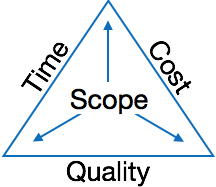
\includegraphics{img/time_cost_quality.png}
    \caption{Tiempo, Costo, Calidad => Alcance}
    \label{fig:triangulo}
\end{figure}

La figura \ref{fig:triangulo} muestra restricciones triples para proyectos de
software, las cuales son tiempo, costo y calidad.\\

Es una parte esencial de la organización del software entregar un producto de 
calidad, manteniendo el costo dentro de las restricciones presupuestarias del 
cliente y entregar el proyecto según lo programado. Hay varios factores, tanto 
internos como externos, que pueden afectar este triángulo de triple restricción. 
Cualquiera de los tres factores puede afectar gravemente a los otros dos.\\

\section{¿Por qué es importante el análisis de riesgos en la administración de 
un proyecto de software?}

Porque al planificar eventos inesperados, se puede estar listo para responder 
si surgen. Para garantizar el éxito del proyecto, hay que definir cómo se 
manejarán los riesgos potenciales para poder identificar, mitigar o evitar 
problemas cuando se necesite. 

\section{Diagrama de Gantt}

\begin{figure}[htb]
    \centering
    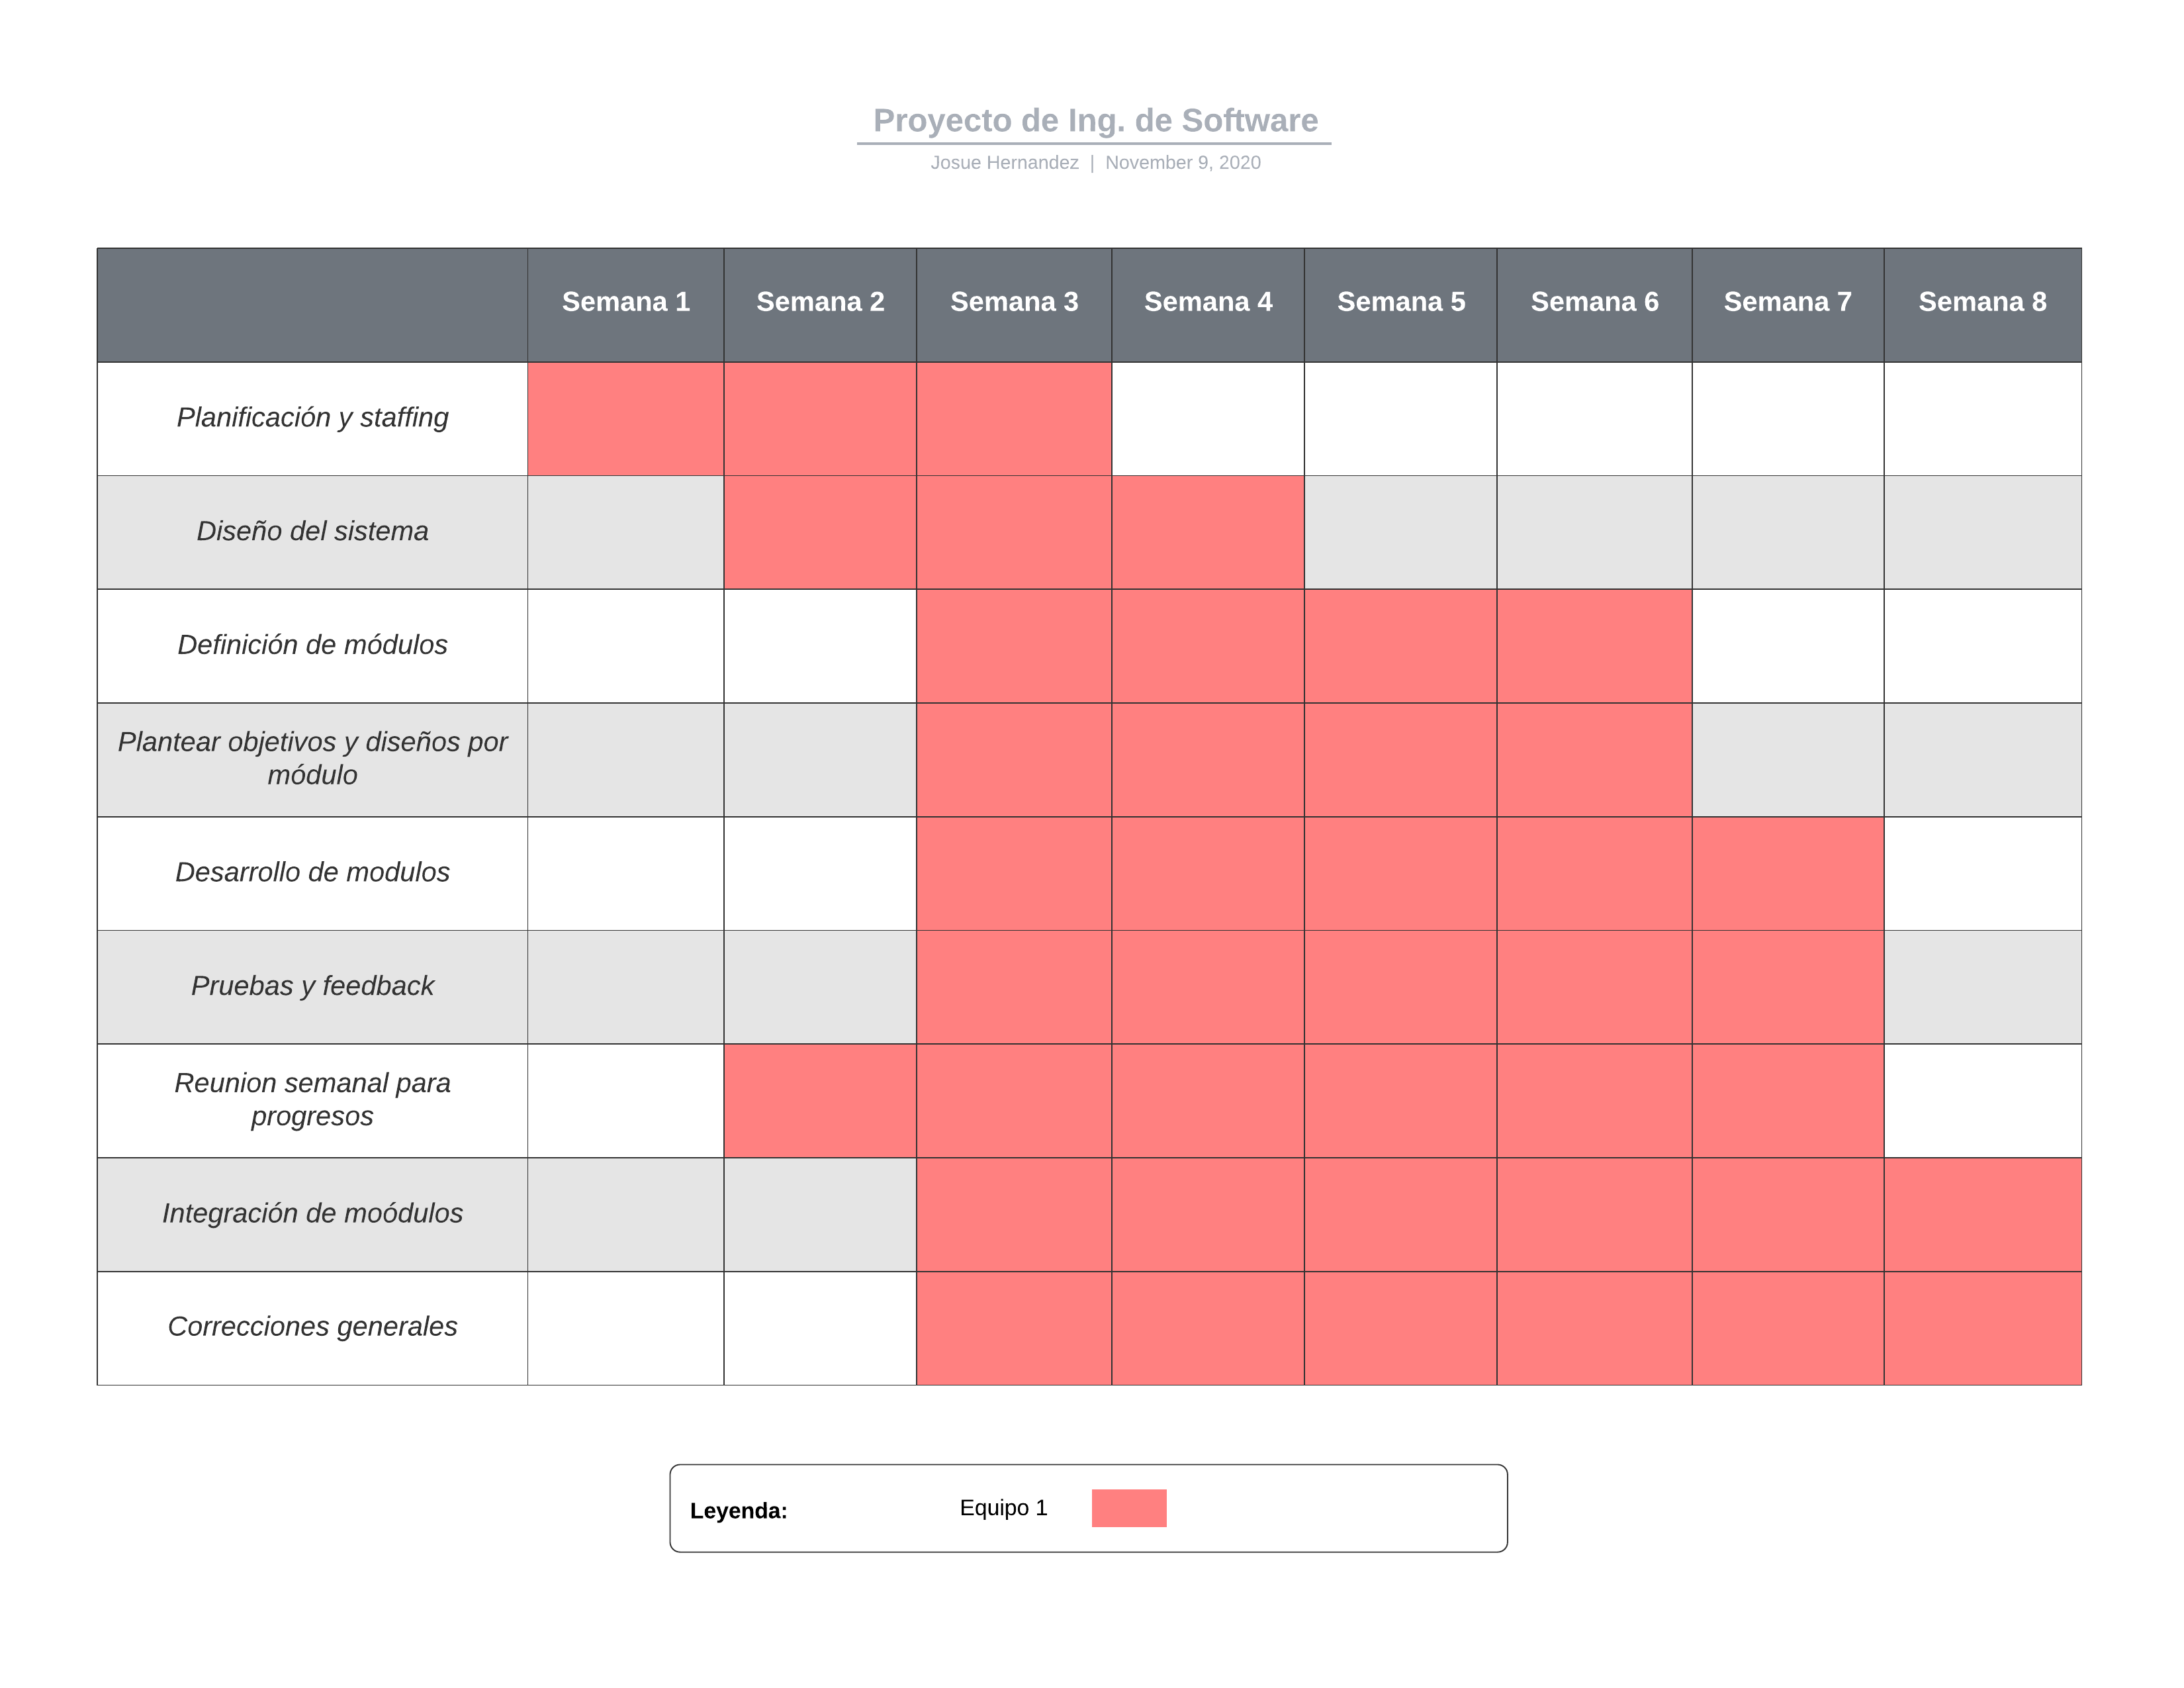
\includegraphics[scale=0.17, angle=90]{img/gantt.png}
    \caption{Planificación personal del proyecto}
    \label{fig:gantt}
\end{figure}

\end{document}

